\documentclass[12pt]{article}

\usepackage[a4paper]{geometry} %page size
\usepackage{parskip} %no paragraph indentation
\usepackage{fancyhdr} %fancy stuff in page header
\pagestyle{fancy} 

\usepackage[utf8]{inputenc} %encoding
\usepackage[danish]{babel} %danish letters

\usepackage{graphicx} %import pictures
\graphicspath{ {images/} }
\usepackage{listings} %make lists

\usepackage{amsmath, amssymb, amsfonts, amsthm, mathtools} %doing math
\usepackage{algorithmicx, algpseudocode} %doing pseudocode

\title{
  Title\
  \large Subtitle
}
\author{Asger Andersen}
\date{\today}

\fancyhead{}
\lhead{Miniprojekt 1}
\rhead{Asger Andersen}

%End of preamble
%*******************************************************************************

\begin{document}

\section*{Introduktion}

Min R-kode er vedlagt som appendix til projektet.

\section{Opgave 1}

\subsection{Delopgave a}

Her er plots af fremskrivningerne af forbrugsmængden $C_t$ og investeringsmængden $I_t$ for $t=1,...,50$:

\begin{center}
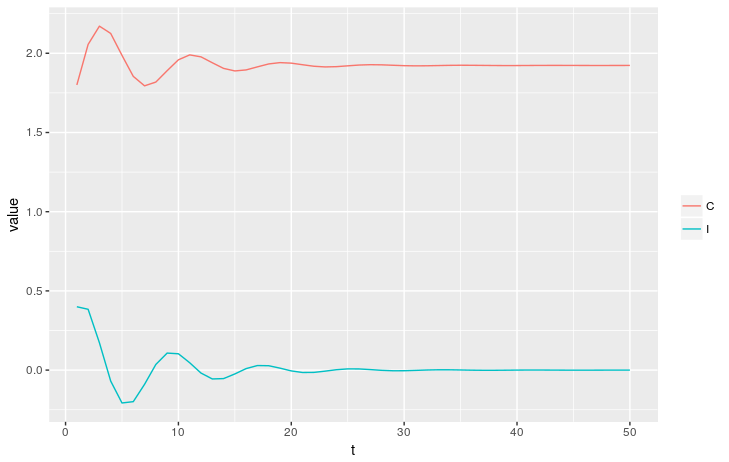
\includegraphics[scale=0.5]{q1p1.png}
\end{center}

Vi ser, at $C_t$ ser ud til at konvergere mod en værdi på lidt mindre end $2$, og $I_t$ ser ud til at konvergere mod $0$, når $t$ går mod uendelig. Her er værdierne af $C_t$ og $I_t$ for $t=45,...,50$:

\begin{table}[ht]
\centering
\begin{tabular}{rrrr}
  \hline
 & t & C & I \\ 
  \hline
1 &      45 & 1.923166 & -0.000291 \\ 
  2 &      46 & 1.922980 & -0.000279 \\ 
  3 &      47 & 1.922897 & -0.000126 \\ 
  4 &      48 & 1.922930 & 0.000050 \\ 
  5 &      49 & 1.923031 & 0.000151 \\ 
  6 &      50 & 1.923127 & 0.000145 \\ 
   \hline
\end{tabular}
\end{table}

Det ser altså ud til, at $(C_t, I_I)$ konveregerer mod $(1.923, 0)$, når $t$ går mod uendelig.

\subsection{Delopgave b, c \& d}

Fra \textbf{sætning B.5.1} ved jeg, at hvis den inverse til matricen 
\begin{align}
(A-E) = \begin{bmatrix}
a-1 && a \\
(a-1)c && ac - 1
\end{bmatrix}
\end{align}
eksisterer, så har modellen netop én ligevægt givet ved
\begin{align}
v^* = 
-(A-E)^{-1}\begin{pmatrix}
b\\
bc
\end{pmatrix}
\end{align}
Da 
\begin{align}
\det (A - E) = (a-1)(ac-1) - a(a-1)c = 1-a
\end{align}
så har $(A-E)$ en invers, hvis og kun hvis $a\neq 1$. I så fald er den inverse givet ved
\begin{align}
(A-E)^{-1} = \frac{1}{1-a} \begin{bmatrix}
ac-1 && -a \\
-(a-1)c && a - 1
\end{bmatrix}
\end{align}
og modellen har netop én ligevægt givet ved
\begin{align}
-(A-E)^{-1}\begin{pmatrix}
b\\
bc
\end{pmatrix} = -\frac{1}{1-a} \begin{bmatrix}
ac-1 && -a \\
-(a-1)c && a - 1
\end{bmatrix}\begin{pmatrix}
b\\
bc
\end{pmatrix} =
\begin{pmatrix}
\frac{b}{1-a}\\
0
\end{pmatrix}
\end{align}
For at finde ud af om denne ligevægt er stabil eller ej, vil jeg se nærmere på egenværdierne for $A$. Jeg opskriver derfor det karakteristiske polynomien for $A$:
\begin{align}
\begin{vmatrix}
a - \lambda && a \\
(a-1)c && ac - \lambda
\end{vmatrix} = \\
(a-\lambda)(ac - \lambda) - a(a-1)c =\\ 
\lambda^2 + (-a(c+1))\lambda + ac
\end{align}

Fra hintet i opgavebeskrivelsen ved jeg, at polynomiet har rødder, der er numerisk skarpt mindre end 1, hvis og kun hvis
\begin{align}
|ac| < 1
\end{align}
og
\begin{align}
|-a(c+1)| < 1 + ac
\end{align}
begge gælder.

Fra \textbf{sætning B.6.2} ved jeg altså, at hvis linje (9) og (10) er opfyldt, så er ligevægten stabil. Alt i alt har jeg nu fundet ud af, at hvis $a\neq 1$ og linje (9) og (10) er opfyldt, så har modellen netop én stabil ligevægt givet ved 
\begin{align}
\begin{pmatrix}
\frac{b}{1-a} \\
0
\end{pmatrix}
\end{align}
I så fald har vi, at uanset hvilken værdi $(C_0, I_0)$ har, så vil $(C_t,I_t)$ konvergere mod denne ligevægt, når $t$ går mod uendelig.

Sætter vi $a=0.48, b=1, c=1.5$, så er $a\neq 1$ og linje (9) og (10) er opfyldt, da
\begin{align}
|ac| = 0.72 < 1
\end{align}
og 
\begin{align}
|-a(c+1)| = 1.2 < 1.72 = 1 + ac
\end{align}
Altså har vores model i så fald netop én stabil ligevægt, og denne er givet ved
\begin{align}
\begin{pmatrix}
\frac{b}{1-a} \\
0
\end{pmatrix}=
\begin{pmatrix}
\frac{1}{1-0.48} \\
0
\end{pmatrix}= 
\begin{pmatrix}
1.9231 \\
0
\end{pmatrix}
\end{align}
Dette svarer til, hvad vi så i den numeriske simulering i delopgave a.

\section{Opgave 2}

\subsection{Delopgave a \& b}

Jeg løser kun delopgave a, da delopgave b ser ud til at blive noget værre regneri, som jeg ikke tør vove mig ud i! For $n=2$ har vi:
\begin{align}
\det(M-\lambda E) =
\begin{vmatrix}
b_0 - \lambda && b_1 && b_2 \\
p_0 && -\lambda && 0 \\
0 && p_1 && -\lambda 
\end{vmatrix} = \\
(b_0 - \lambda) \begin{vmatrix}
-\lambda && 0 \\
p_1 && -\lambda  
\end{vmatrix} - b_1 \begin{vmatrix}
p_0 && 0 \\
0 && -\lambda  
\end{vmatrix} + 
b_2 \begin{vmatrix}
p_0 && -\lambda \\
0 && p_1  
\end{vmatrix} = \\
(b_0 - \lambda)\lambda^2 
+ b_1p_0\lambda  + 
b_2 p_0 p_1 = \\
-(\lambda^3 - \l_0b_0\lambda^2 - l_1b_1\lambda - l_2 b_2)
\end{align}

\subsection{Delopgave c}

Fra opgavetekstens formular for $\det(M-\lambda E)$ for vilkaarligt $n$ har vi:
\begin{align}
\det(M-\lambda E) = (-1)^{n+1}\left(\lambda^{n+1} - \sum_{i=0}^n l_ib_i\lambda^{n-i} \right)
\end{align}
Altsaa gaelder det at
\begin{align}
\det(M-\lambda E) = 0
\end{align}
hvis og kun hvis
\begin{align}
 (-1)^{n+1}\left(\lambda^{n+1} - \sum_{i=0}^n l_ib_i\lambda^{n-i} \right) = 0
\end{align}
hvis og kun hvis
\begin{align}
\sum_{i=0}^n l_ib_i\lambda^{n-i} = \lambda^{n+1}
\end{align}
hvis og kun hvis
\begin{align}
\sum_{i=0}^n l_ib_i\lambda^{-(i+1)} = 1
\end{align}
hvilket per definition af $S(\lambda)$ vil sige, hvis og kun hvis
\begin{align}
S(\lambda) = 1
\end{align}
Altså har vi nu vist, at 
\begin{align}
\det(M-\lambda E) = 0
\end{align}
hvis og kun hvis 
\begin{align}
S(\lambda) = 1
\end{align}
Per definition af egenværdier vil det sige, at $\lambda$ er egenværdi for $M$, hvis og kun hvis $S(\lambda)=1$.

Jeg vil nu vise, at $M$ har netop én skarpt positiv egenværdi. 

Lad os definere 
\begin{align}
f_i(\lambda) = l_ib_i\lambda^{-(i+1)}, \quad i\in\mathbb{N}_0
\end{align}

Da gaelder
\begin{align}
S(\lambda) = \sum_{i=0}^n f_i(\lambda)
\end{align}

Lad $\lambda>0$. Da ser vi, at $f_i$ en positiv, aftagende funktion for alle $i\in \mathbb{N}_0$. Altsaa er $S$ en sum af positive, aftagende funktioner og er altsaa selv positiv og aftagende. Vi ser ydermere, at for alle $i \in \mathbb{N}_0$ gaelder, at $f_i(\lambda) \to \infty$ for $\lambda \to 0_+$ og $f_i \to 0$ for $\lambda \to \infty$. Da graensevaerdier distribuerer over summer, har vi altsaa 
\begin{align}
\lim_{\lambda \to 0_+} S(\lambda) = \sum_{i=0}^n \lim_{\lambda \to 0_+} f_i(\lambda) =  \sum_{i=0}^n \infty = \infty 
\end{align}
og
\begin{align}
\lim_{\lambda \to \infty} S(\lambda) = \sum_{i=0}^n \lim_{\lambda \to \infty} f_i(\lambda) =  \sum_{i=0}^n 0 = 0
\end{align}
$S(\lambda)$ vil have omtrentligt samme form som $\lambda^{-1}$. Her er en skitse af den omtrentlige form af $S$ for $\lambda>0$:
\begin{center}
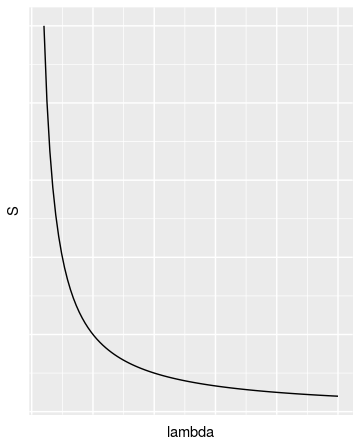
\includegraphics[scale=0.5]{q2Splt.png}
\end{center}
Lad mig nu argumentere for, at der eksisterer netop ét $\lambda_1 >0$, saa $S(\lambda_1)=1$. Eftersom $f_i(\lambda)$ er kontinuert over $\lambda > 0$ for alle $i\in \mathbb{N}_0$, saa er $S$ en sum af kontinuerte funktioner og altsaa selv kontinuert over $\lambda >0$. Da $S$ graenser mod uendelig, naar $\lambda$ gaar mod 0, og mod 0 naar $\lambda$ gaar mod uendelig, saa ved vi, at der maa eksisterer mindst ét $\lambda_1$ i $(0, \infty)$, saa $S(\lambda_1)=1$. Da $S$ er aftagende paa $(0, \infty)$, saa ved vi yderligere, at der hoejst kan eksiterere ét $\lambda_1$ i $(0, \infty)$, saa $S(\lambda_1) =1$. Altsaa eksisterer der netop ét $\lambda_1$ i $(0, \infty)$, saa $S(\lambda_1) =1$.

Eftersom $\lambda>0$ er egenvaerdi for $M$, hvis og kun hvis $S(\lambda)=1$, saa har vi nu alt i alt vist, at $M$ har netop én positiv egenvaerdi.

\subsection{Delopgave d}

Fra definitionen af $M$ er det klart, at $M$ er ikke-negativ. Hvis vi desuden antager, at $M^{n+1}$ er positiv, så kan vi bruge Perron-Frobenius' sætning 3 til at konkludere, at $M$ har en positiv, dominerende egenværdi. Eftersom vi ved fra delopgave c, at $M$ kun har én positiv egenværdi, nemlig $\lambda_1$, må $\lambda_1$ altså være dominerende egenværdi for $M$.

\subsection{Delopgave e}

Definer vektoren $q\in \mathbb{R}^{n+1}$ koordinatvis ved
\begin{align}
q_i = l_{i}\lambda_1^{-i}, \qquad i=0,...,n
\end{align}
hvor vi har nul-indekseret $q$. Hermed kan vi også udregne vektoren $\lambda_1q\in \mathbb{R}^{n+1}$ koordinatvis som 
\begin{align}
(\lambda_1 q)_i = \lambda_1l_{i}\lambda_1^{-i} = l_{i}\lambda_1^{1-i}, \qquad i=0,...,n
\end{align}
Lad os nu udregne koordinaterne af vektoren $Mq\in \mathbb{R}^{n+1}$. Det i'te koordinat er per definition af matrix produkter lig prikproduktet af den i'te række af $M$ og $q$:
\begin{align}
(Mq)_i = (M_{i,\cdot})\cdot q, \qquad i=0,...,n
\end{align}
Her har vi også nul-indekseret rækkerne i $M$. 

Jeg vil nu regne lidt på disse prikprodukter. Lad først $i=0$. Hermed har vi:
\begin{align}
(M_{i,\cdot})\cdot q = 
\sum_{j=0}^n b_j q_j = \sum_{j=0}^n b_jl_j\lambda_1^{-j}
\end{align}
Lad nu $i\in \{1,...,n\}$. Da har vi:
\begin{align}
(M_{i,\cdot})\cdot q = 
p_{i-1}q_{i-1} = \\ 
p_{i-1}l_{i-1}\lambda_1^{-(i-1)} = \\ 
p_{i-1}(p_0p_1...p_{i-2}) \lambda_1^{1-i} = \\
(p_0p_1...p_{i-2}p_{i-1}) \lambda_1^{1-i} = \\
l_i \lambda_1^{1-i}
\end{align}

Vi har per definition af egenvektorer, at $q$ er en egenvektor for $M$ hørende  til $\lambda_1$, hvis og kun hvis
\begin{align}
\forall i \in \{0,...,n\}:\  (Mq)_i = (\lambda_1q)_i
\end{align}
Fra linje (32), (32) og (35-39) får vi
\begin{align}
\forall i \in \{1,...,n\}:\  (Mq)_i = (\lambda_1q)_i
\end{align}
Hermed mangler vi kun at vise, at
\begin{align}
(Mq)_0 = (\lambda_1q)_0
\end{align}

Linje (32), (33) og (34) giver, at linje (42) er sand, hvis og kun hvis
\begin{align}
\sum_{j=0}^n b_jl_j\lambda_1^{-j} = l_{0}\lambda_1^{1-0} = \lambda_1
\end{align}
hvilket er ækvivalent med 
\begin{align}
\sum_{j=0}^n b_jl_j\lambda_1^{-(j+1)} = 1
\end{align}
hvilket er det samme som
\begin{align}
S(\lambda_1)=1
\end{align}
Dette gælder for enhver egenværdi for $M$ og derfor også for $\lambda_1$. Altså gælder
\begin{align}
(Mq)_0 = (\lambda_1q)_0
\end{align}
Altså har vi nu alt i alt vist, at $q$ er en egenvektor for $M$ hørende til egenværdien $\lambda_1$.

\section{Opgave 3}

\subsection{Delopgave a}

Her er et plot af fremskrivningen af antallet af individer i de tre aldersgrupper for $t=0,..,10$:
\begin{center}
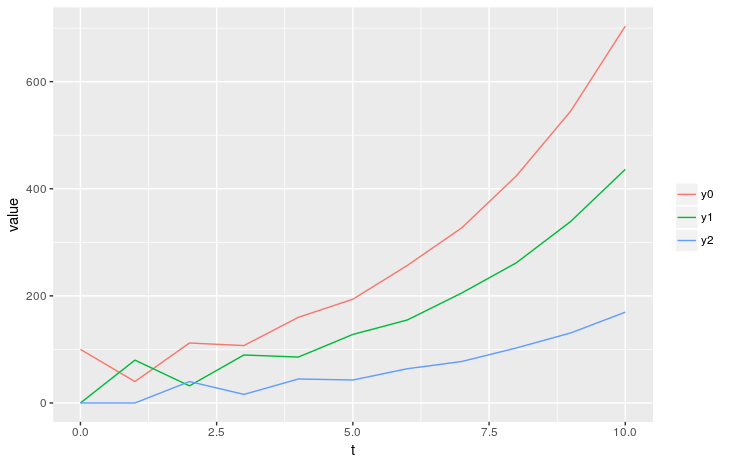
\includegraphics[scale=0.5]{q3p1.png}
\end{center}
og for $t=0,...,30$:
\begin{center}
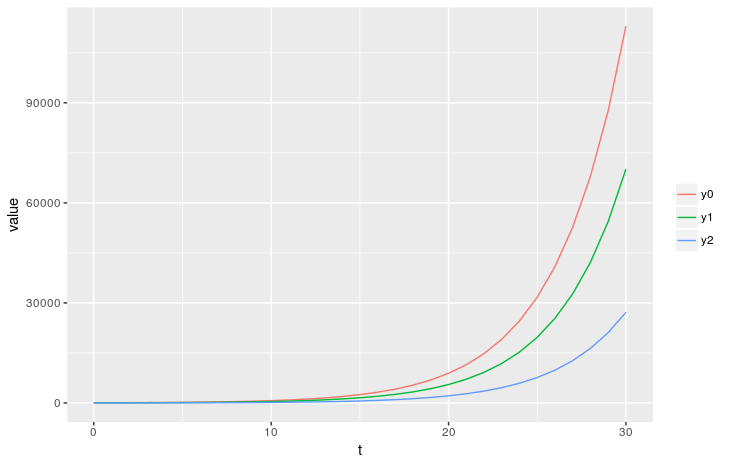
\includegraphics[scale=0.5]{q3p2.png}
\end{center}

Her er et plot af fremskrivningen af vækstraten for de tre aldersgrupper for $t=0,..,20$:
\begin{center}
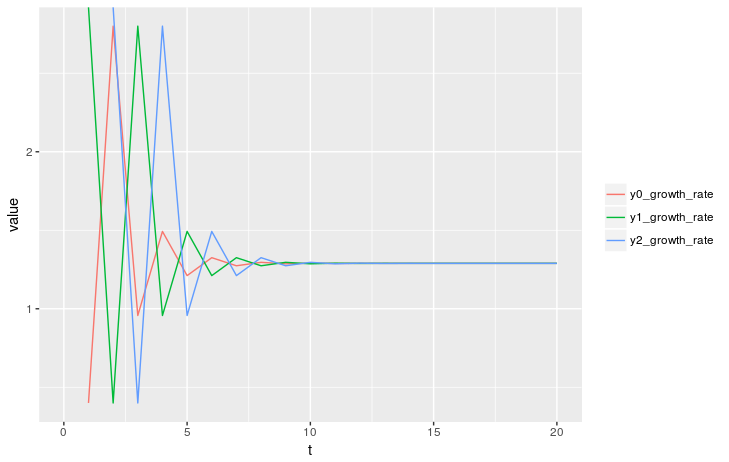
\includegraphics[scale=0.5]{q3p4.png}
\end{center}
Modellen ser ud til en dominerende egenværdi på omkring $\lambda_1=1.3$.

Her er et plot af fremskrivningen af procentfordelingen af tre aldersgrupper for $t=0,..,20$:
\begin{center}
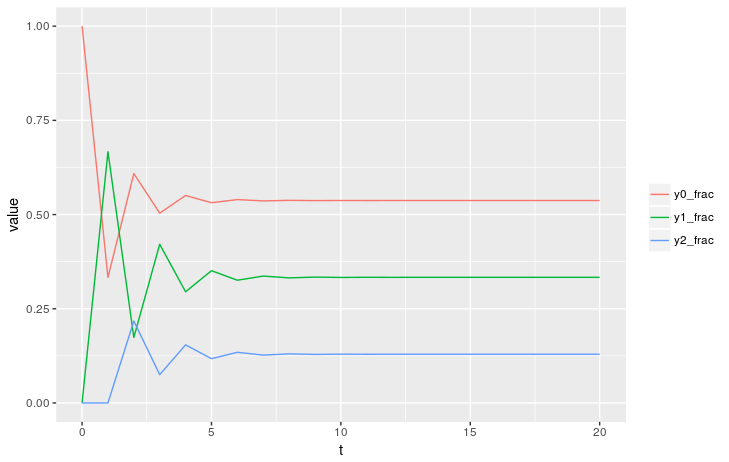
\includegraphics[scale=0.5]{q3p3.png}
\end{center}
Modellen ser ud til at have en egenvektor hørende til $\lambda_1$ med værdier omkring $q=(0.54, 0.33, 0.13)$.

\subsection{Delopgave b}

Her er et plot af $S(\lambda)$ for vores konkrete model:
\begin{center}
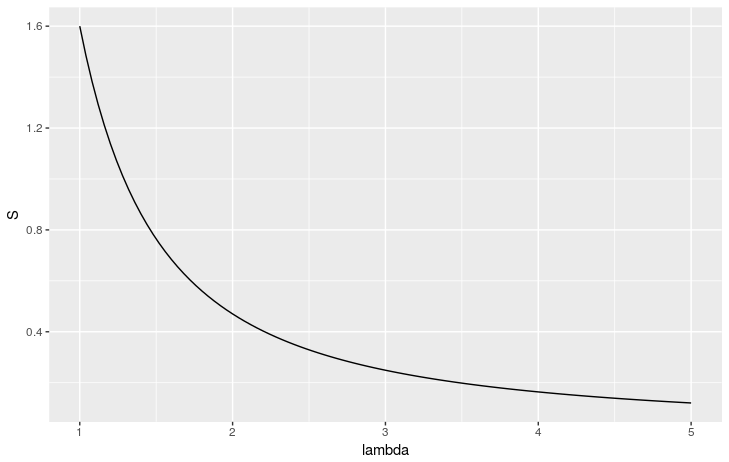
\includegraphics[scale=0.5]{q3p5.png}
\end{center}

Som forventet fra besvarelsen af opgave 2, ser vi at $S(\lambda)$ er aftagende og er lig 1 for netop ét $\lambda_1$. Fra opgave 2 ved vi, at dette $\lambda_1$ er den søgte dominerende egenværdi for vores model.

Ved hjælp af uniroot finder jeg $\lambda_1=1.29$.

\subsection{Delopgave c}

Ved hjælp af eigen funktionen i R finder jeg, at vores model har egenværdierne $(1.29, -0.55, -0.34)$ og tilhørende matrix af egenvektorer
\begin{align}
Q =
\begin{bmatrix}
0.83 & -0.45 & 0.23 \\ 
  0.52 & 0.66 & -0.54 \\ 
  0.20 & -0.60 & 0.81
\end{bmatrix}
\end{align}
R finder ikke den egenvektor $(0.54,0.33,0.13)$ hørende til $\lambda_1$, som jeg foreslog ovenfor ud fra fremskrivningen. Det er fordi R finder en egenvektor med norm 1, hvilket vektoren $(0.54,0.33,0.13)$ ikke har. Dog ligger vektorene i samme underrum, da $(0.54,0.33,0.13) = 0.65(0.83, 0.52, 0.2)$. Altså finder R blot en anden vektor i egenrummet for $\lambda_1$.

Når jeg udregner $Q^{-1}MQ$ i R, får jeg som forventet en diagonalmatrix med egenværdierne $(1.29, -0.55, -0.34)$ i diagonalen.


\subsection{Delopgave d}

Jeg viser det ønskede for det $n$-dimensionelle tilfælde, da jeg ikke synes, at det forøger bevisets kompleksitet væsentligt.

Lad $M$ være en $n$-dimensionel matrix med $n$ forskellige egenværdi $\lambda_1, ..., \lambda_n$, hvor $\lambda_1$ er den dominerende egenværdi. Lad $q_i$ være en egenvektor tilhørende egenværdien $\lambda_i$ for $i=1,...,n$. 

Lad $v_0\in\mathbb{R}^n$. Eftersom alle egenværdierne for $M$ er forskellige, udgør $q_1,...,q_n$ en basis for $\mathbb{R}^n$. Altså kan vi dekomponerer $v_0$ som en vægtet sum af egenvektorerne
\begin{align}
v_0 = \sum_{i=1}^n c_iq_i,\qquad c_1,...,c_n\in \mathbb{R}
\end{align}
Vi har altså
\begin{align}
v_t = M^tv_0 = M_t\sum_{i=1}^n c_iq_i = \sum_{i=1}^n c_iM^tq_i 
\end{align}
Vi har, at 
\begin{align}
M^1q_i = \lambda_i^1 q_i 
\end{align}
og antager vi, at
\begin{align}
M^{t-1}q_i= \lambda_i^{t-1}q_i
\end{align}
foelger det direkte, at 
\begin{align}
M^tq_i = M(M^{t-1}q_i)= M(\lambda_i^{t-1}q_i) = \lambda_i^{t-1}(Mq_i) = \lambda_i^tq_i
\end{align}
Altsaa har vi per induktion, at for alle $t\in\mathbb{N}$
\begin{align}
M^tq_i= \lambda_i^tq_i
\end{align}
Altsaa har vi nu alt i alt vist, at 
\begin{align}
v_t = \sum_{i=1}^n c_iM^tq_i = \sum_{i=1}^n c_i\lambda_i^tq_i
\end{align}
Hermed foelger det, at
\begin{align}
\lim_{t\to \infty} \frac{1}{\lambda_1^t}v_t = \lim_{t\to \infty} \frac{1}{\lambda_1^t} \sum_{i=1}^n c_i\lambda_i^tq_i = \sum_{i=1}^n c_i q_i \lim_{t\to \infty} \left( \frac{\lambda_i}{\lambda_1} \right)^t
\end{align}
Da $\lambda_1$ er dominerende egenværdi, saa er $\lambda_i<\lambda_1$ for alle $i=2,...,n$. Altsaa har vi
\begin{align}
\lim_{t\to \infty} \left( \frac{\lambda_i}{\lambda_1} \right)^t = \begin{cases}
1, & i=1 \\
0, & i\neq 1 
\end{cases}
\end{align}
Altsaa har vi alt i alt, at
\begin{align}
\lim_{t\to \infty} \frac{1}{\lambda_1^t}v_t = c_1q_1
\end{align}

\subsection{Delopgave e}

Definer funktionen
\begin{align}
S_a(\lambda) = \frac{0.4}{\lambda} + \frac{0.8a}{\lambda^2} + \frac{0.24}{\lambda^3}
\end{align}
Da $S_a$ er aftagende, har den en invers, og vi ved fra opgave 2, at den inverse til 1 er den dominerende egenværdi $\lambda_1$:
\begin{align}
S_a^{-1}(1)=\lambda_1
\end{align}
Da $\lambda_1$ er den vækstrate, som populationen konvergere imod, vil populationen uddø på lang sigt, hvis og kun hvis $\lambda_1<1$. Altså kan vi vi betragte mængden af relle tal $a$, som vil få populationen til at overleve på lang sigt:
\begin{align}
A = \{a\in \mathbb{R}\ |\ 1 \leq S_a^{-1}(1) \}
\end{align}
Vi skal altså bestemme minimum af denne mængde. 

Her er et plot af $f(a) = S_a^{-1}(1)$, som jeg har udregnet numerisk i R:
\begin{center}
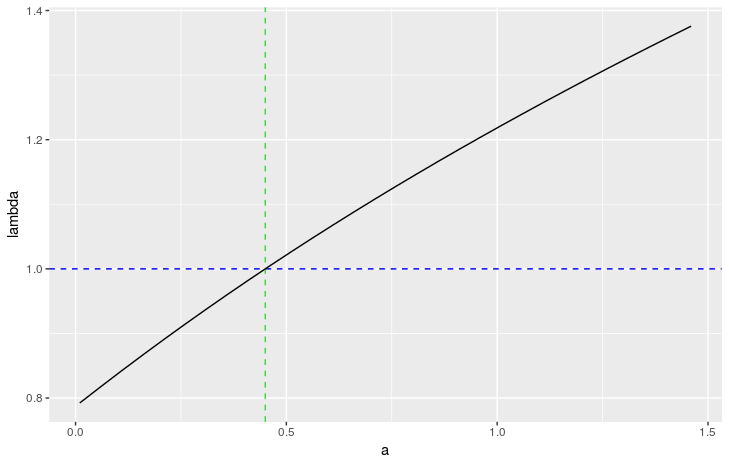
\includegraphics[scale=0.5]{q3p6.png}
\end{center}
På plottet svarer mængden $A$, som jeg lige har defineret den, til alle de $a$, der ligger på og til højre for den grønne linje. Vi ser, at $f(a)$ er en voksende funktion af $a$, hvilket giver god mening, da $f(a)$ jo netop er den langsigtede vækstrate givet $b_1=a$, og jo større $b_1$ er, jo større burde den langsigtede vækstrate også være. Da $f(a)$ er en voksende funktion af $a$, så er minimum af mængden $A$ det ene element, der opfylder
\begin{align}
\{a\in \mathbb{R}\ |\ 1 = S_a^{-1}(1) \}
\end{align}
Ved hjælp af uniroot bestemmer jeg numerisk dette element til at være lig 0.45. Altså vil populationen overleve på lang sigt, hvis og kun hvis $0.45\leq a$.

\end{document}